%%%%%%%%%%%%%%%%%%%%%%%%%%%%%
% Standard header for working papers
%
% WPHeader.tex
%
%%%%%%%%%%%%%%%%%%%%%%%%%%%%%

\documentclass[11pt]{article}

%%%%%%%%%%%%%%%%%%%%
%% Include general header where common packages are defined
%%%%%%%%%%%%%%%%%%%%

% general packages without options
\usepackage{amsmath,amssymb,bbm}




%%%%%%%%%%%%%%%%%%%%
%% Idem general commands
%%%%%%%%%%%%%%%%%%%%
%% Commands

\newcommand{\noun}[1]{\textsc{#1}}


%% Math

% Operators
\DeclareMathOperator{\Cov}{Cov}
\DeclareMathOperator{\Var}{Var}
\DeclareMathOperator{\E}{\mathbb{E}}
\DeclareMathOperator{\Proba}{\mathbb{P}}

\newcommand{\Covb}[2]{\ensuremath{\Cov\!\left[#1,#2\right]}}
\newcommand{\Eb}[1]{\ensuremath{\E\!\left[#1\right]}}
\newcommand{\Pb}[1]{\ensuremath{\Proba\!\left[#1\right]}}
\newcommand{\Varb}[1]{\ensuremath{\Var\!\left[#1\right]}}

% norm
\newcommand{\norm}[1]{\| #1 \|}


% amsthm environments
\newtheorem{definition}{Definition}



%% graphics

% renew graphics command for relative path providment only ?
%\renewcommand{\includegraphics[]{}}








% geometry
\usepackage[margin=2cm]{geometry}

% layout : use fancyhdr package
\usepackage{fancyhdr}
\pagestyle{fancy}

\makeatletter

\renewcommand{\headrulewidth}{0.4pt}
\renewcommand{\footrulewidth}{0.4pt}
%\fancyhead[RO,RE]{\textit{Working Paper}}
\fancyhead[RO,RE]{\textit{ECTQG 2015}}
%\fancyhead[LO,LE]{G{\'e}ographie-Cit{\'e}s/LVMT}
\fancyhead[LO,LE]{An Algorithmic Systematic Review}
\fancyfoot[RO,RE] {\thepage}
\fancyfoot[LO,LE] {\noun{J. Raimbault}}
\fancyfoot[CO,CE] {}

\makeatother


%%%%%%%%%%%%%%%%%%%%%
%% Begin doc
%%%%%%%%%%%%%%%%%%%%%

\begin{document}







\title{Génération de Données Synthétiques Corrélées\\\medskip
\textit{Actes des Journées de Rochebrune 2016}
}
\author{\noun{Juste Raimbault}$^{1,2}$\\
$^{1}$ UMR CNRS 8504 Géographie-cités\\
$^{2}$ UMR-T IFSTTAR 9403 LVMT
}
\date{date}


\maketitle

\justify


\begin{abstract}
\end{abstract}



%%%%%%%%%%%%%%%%%%%%%%
\section{Introduction}
%%%%%%%%%%%%%%%%%%%%%%

L'utilisation de données synthétiques, au sens de populations statistiques d'individus générées aléatoirement sous la contrainte de reproduire certaines caractéristiques du système étudié, est une pratique méthodologique largement répandue dans de nombreuses disciplines, et particulièrement pour des problématiques liées aux systèmes complexes, telles que par exemple l'évaluation thérapeutique~\cite{abadie2010synthetic}, l'étude des systèmes territoriaux~\cite{moeckel2003creating,pritchard2009advances}, l'apprentissage statistique~\cite{bolon2013review} ou la bio-informatique~\cite{van2006syntren}. Il peut s'agir d'une désagrégation par création d'une population au niveau microscopique présentant des caractéristiques macroscopiques données, ou bien de la création de nouvelles populations au même niveau d'agrégation qu'un échantillon donné avec un critère de ressemblance aux données réelles. Le niveau de ce critère peut % find minimal common characteristics ?
% TODO generalization of data proximity

Les intérêts de ces méthodes sont directement liés 



Si le premier ordre est bien maitrisé, il n'a à notre connaissance pas été proposé de méthode systématique permettant un contrôle au second ordre,% rq correlated choices in DC model ?
c'est à dire où la structure de correlation estimée sur les données générées est maitrisée. Nous proposons une telle méthode ainsi que son application à deux exemples de systèmes complexes dans des domaines relativement éloignés.

La suite de l'article est organisée de la façon suivante : 


%%%%%%%%%%%%%%%%%%%%%%
\section{Formalisation de la méthode}
%%%%%%%%%%%%%%%%%%%%%%

L'ensemble des méthodologies mentionnées en introduction sont trop variées pour être résumées par un même formalisme. Nous proposons ici une formulation générique ne dépendant pas du domaine d'application, ciblée sur le contrôle de la structure de correlation des données synthétiques.

Soit un processus stochastique multidimensionnel $\vec{X}_I$ (l'ensemble d'indexation pouvant être par exemple le temps dans le cas de séries temporelles, l'espace, ou l'indexation). On se propose, à partir d'un jeu de réalisations $\mathbf{X}=(X_{i,j})$, de générer une population statistique $\mathbf{\tilde{X}}=\tilde{X}_{i,j}$ telle que
\begin{itemize}
\item d'une part un certain critère de proximité aux données est vérifié, i.e. étant donné une précision $\varepsilon$ et un indicateur $f$, $\norm{f(\mathbf{X})-f(\mathbf{\tilde{X}})} < \varepsilon$
\item d'autre part le niveau de correlation est controlé, i.e. étant donné une matrice fixant une structure de covariance $R$, $\Varb{(\tilde{X}_i)} = R$, où la matrice de variance/covariance est estimée sur la population synthétique.
\end{itemize}


%%%%%%%%%%%%%%%%%%%%%%
\section{Applications}
%%%%%%%%%%%%%%%%%%%%%%



%%%%%%%%%%%%%%%%%%%%%%
\subsection{Application : séries temporelles financières}


%%%%%%%%%%%%%%%%%%%%%%
\subsubsection{Contexte}

Un premier domaine d'application proposé pour notre méthode est celui des séries temporelles financières, signaux typiques de systèmes complexes hétérogènes et multiscalaires~\cite{mantegna2000introduction} et pour lesquels les corrélations ont fait l'objet d'abondants travaux. Ainsi, l'application de la théorie des matrices aléatoires peut permettre de débruiter, ou du moins d'estimer la part de signal noyée dans le bruit, une matrice de correlations pour un grand nombre d'actifs échantillonnés à faible fréquence (retours journaliers par exemple)~\cite{2009arXiv0910.1205B}. De même, l'analyse de réseaux complexes construits à partir des corrélations, selon des méthodes type arbre couvrant minimal~\cite{2001PhyA..299...16B} ou des extensions raffinées pour cette application précise~\cite{tumminello2005tool}, ont permis d'obtenir des résultats prometteurs, tels la reconstruction de la structure économique des secteurs d'activités. A haute fréquence, l'estimation précise de paramètres d'interdépendance dans le cadre d'hypothèses fixées sur la dynamique, fait l'objet d'importants travaux théoriques dans un but de raffinement des modèles et des estimateurs~\cite{barndorff2011multivariate}. Les résultats théoriques doivent alors être testés sur des jeux de données synthétiques, qui permettent de contrôler un certain nombre de paramètres et de s'assurer qu'un effet prédit par la théorie est bien observable \emph{toutes choses égales par ailleurs}. Par exemple, \cite{potiron2015estimation} dérive une correction du biais de l'estimateur de \emph{Hayashi-Yoshida} qui est un estimateur de la covariance de deux browniens corrélés à haute fréquence dans le cas de temps d'observation asynchrones, par démonstration d'un théorème de la limite centrale pour un modèle généralisé endogénéisant les temps d'observations. La confirmation empirique de l'amélioration de l'estimateur est alors obtenue sur un jeu de données synthétiques à un niveau de corrélation fixé.


%%%%%%%%%%%%%%%%%%%%%%
\subsubsection{Formalisation}

\paragraph{Cadre}

Considérons un réseau d'actifs $(X_i(t))_{1\leq i \leq N}$ échantillonnés à haute fréquence (typiquement 1s). On se place dans un cadre multi-scalaire (utilisé par exemple dans les approches par ondelettes~\cite{ramsey2002wavelets} ou analyses multifractales du signal~\cite{bouchaud2000apparent}) pour interpréter les signaux observés comme la superposition de composantes à des multiples échelles temporelles : $X_i=\sum_{\omega}{X_i^{\omega}}$. Prédire l'évolution d'une composante à une échelle donnée est alors un problème caractéristique de l'étude des systèmes complexes, pour lequel l'enjeu est l'identification de régularités et leur distinction des composantes considérées comme stochastiques en comparaison. Dans un souci de simplicité, on représente un tel processus par un modèle de prédiction de tendance à une échelle temporelle $\omega_1$ donnée, formellement un estimateur $M_{\omega_1} : (X_i(t'))_{t'<t} \mapsto \hat{X_i}(t)$ dont l'objectif est la minimisation de l'erreur sur la tendance réelle $\norm{X_i^{\omega}}$. Dans le cas d'estimateurs auto-regressifs multivariés, la performance dépendra entre autre des correlations respectives entre actifs et il est alors intéressant d'utiliser la méthode pour évaluer celle-ci en fonction de niveaux de correlation à plusieurs échelles. On assume une dynamique de Black-Scholes~\cite{jarrow1999honor} pour les actifs, i.e. $dX = \sigma\cdot dW$ avec $W$ processus de Wiener, ce qui permettra d'obtenir facilement des niveaux de correlation voulus.

\paragraph{Génération des données}

Il est alors aisé de générer $\tilde{X}_i$ tel que $\Varb{\tilde{X}_i^{\omega_0}}=\Sigma R$ ($\Sigma$ variance estimée et $R$ matrice de corrélation fixée), par la simulation de processus de Wiener au niveau de corrélation fixé et tel que $X_i^{\omega < \omega_0} = \tilde{X}_i^{\omega < \omega_0}$ (critère de proximité au données : les composantes à plus basse fréquence sont identiques). En effet, si $dW_1 \indep dW_1^{\indep}$, alors $W_2 = \rho_{12}W_1 + \sqrt{1-\frac{\sigma_1^2}{\sigma_2^2}\cdot\rho_{12}^2}W_1^{\indep}$ est tel que $\rho(dW_1,dW_2)=\rho_{12}$. Les signaux suivants sont construits de la même manière par orthonormalisation de Gram. On isole alors la composante de la première fréquence $\omega_1 < \omega_0$ par filtrage, et on reconstruit les signaux synthétiques par $\tilde{X}_i = [\sum_{\omega<\omega_1}X_i^{\omega}]+\tilde{X}_i^{\omega_0}$.
% TODO pb signal reconstruction, clarify formalisation.


\subsubsection{Implémentation et Résultats}

\paragraph{Méthodologie}

La méthode est testée sur un exemple de deux actifs du marché des devises (EUR/USD et EUR/GBP), sur une période de 6 mois de juin 2015 à novembre 2015. Le nettoyage des données\footnote{obtenues depuis \texttt{http://www.histdata.com/}, sans licence spécifiée, les données nettoyées et filtrées à $\omega_m$ uniquement sont mises en accessibilité pour respect du copyright.}, originellement échantillonnées à l'ordre de la seconde, consiste dans un premier temps à la détermination du support temporel commun maximal (les séquences manquantes étant alors ignorées, par translation verticale des séries, i.e. $S(t):=S(t)\cdot \frac{S(t_{n})}{S(t_{n-1})}$ lorsque $t_{n-1},t_n$ sont les extrémités du ``trou'' et $S(t)$ la valeur de l'actif, ce qui revient à garder la contrainte d'avoir des retours à pas de temps similaires entre actifs). On étudie alors les \emph{log-prix} et \emph{log-retours}, définis par $X(t):=\log{\frac{S(t)}{S_0}}$ et $\Delta X (t) = X(t) - X(t-1)$. Les données brutes sont filtrées à une fréquence $\omega_m = 10\textrm{min}$ (qui sera la fréquence maximale d'étude) pour un souci de performance computationnelle. On fixe $\omega_0=12\textrm{h}$ et on se propose de construire des données synthétiques aux fréquences $\omega_1 = 30\textrm{min},1\textrm{h},2\textrm{h}$. Il est crucial de noter l'interférence entre les fréquences $\omega_0$ et $\omega_1$ dans le signal construit : la correlation effectivement estimée est
\[
\rho_{e} = \rho \left[ \Delta \tilde{X}_1 , \Delta \tilde{X}_2 \right] = \rho \left[ \Delta X_1^{\omega_0} + \sum_{\omega_0 < \omega < \omega_1} \Delta \tilde{X}_1^{\omega} , \Delta X_2^{\omega_0} + \sum_{\omega_0 < \omega < \omega_1} \Delta \tilde{X}_2^{\omega}\right]
\]
ce qui conduit à dériver dans la limite raisonnable $\sigma_1 \gg \sigma_0$ (fréquence fondamentale suffisamment basse), lorsque $\Covb{\tilde{X}_i^{\omega}}{X_j^{\omega_0}}=0$ pour tous $i,j,\omega > \omega_0$, et les retours d'espérance nulle à toutes échelles, en notant $\rho_0 = \rho \left[ \Delta X_1^{\omega_0} , \Delta X_2^{\omega_0} \right]$, $\rho = \rho \left[ \sum_{\omega_0 < \omega < \omega_1} \tilde{X}_1^{\omega} , \sum_{\omega_0 < \omega < \omega_1} \tilde{X}_2^{\omega} \right]$, et $\varepsilon_i = \frac{\sigma (X_i^{\omega_0})}{\sigma \left( \sum_{\omega_0 < \omega < \omega_1} \tilde{X}_i^{\omega}\right)}$, la correction sur la correlation effective due aux interférences : la correlation effective est alors au premier ordre

\begin{equation}
\label{eq:eff_corr}
\rho_e = \left[ \varepsilon_1 \varepsilon_2 \rho_0 + \rho \right] \cdot \left[ 1 - \frac{1}{2}\left(\varepsilon_1^2 + \varepsilon_2^2 \right) \right]
\end{equation}

ce qui donne l'expression de la correlation que l'on pourra effectivement simuler dans les données synthétiques



% TODO : explain which estimator

% TODO : formalize arma model.


\paragraph{Implémentation}

L'implémentation est faite en language R, utilisant en particulier la bibliothèque \texttt{MTS}~\cite{Tsay:2015xy} pour les modèles de séries temporelles. Les données nettoyées et le code source sont disponibles de manière ouverte sur le dépôt \texttt{git} du projet\footnote{at \texttt{https://github.com/JusteRaimbault/SynthAsset}}.

\paragraph{Résultats}

La figure~\ref{fig:effective_corrs} donne les correlations effectives calculées sur les données synthétiques.
% comment

Pour des valeurs standard des paramètres (par exemple pour $\omega_0=24\textrm{h}$, $\omega_1=2\textrm{h}$ et $\rho=-0.5$, on a $\rho_0\simeq 0.71$ et $\varepsilon_i \simeq 0.3$ et ainsi $\left| \rho_e - \rho \right|\simeq 0.13$)

% fig:model_perf : application à la perf de l'arma.

% implication thématiques et développements possibles


%%%%%%%%%%%%%%%%%%%
\begin{figure}
\centering
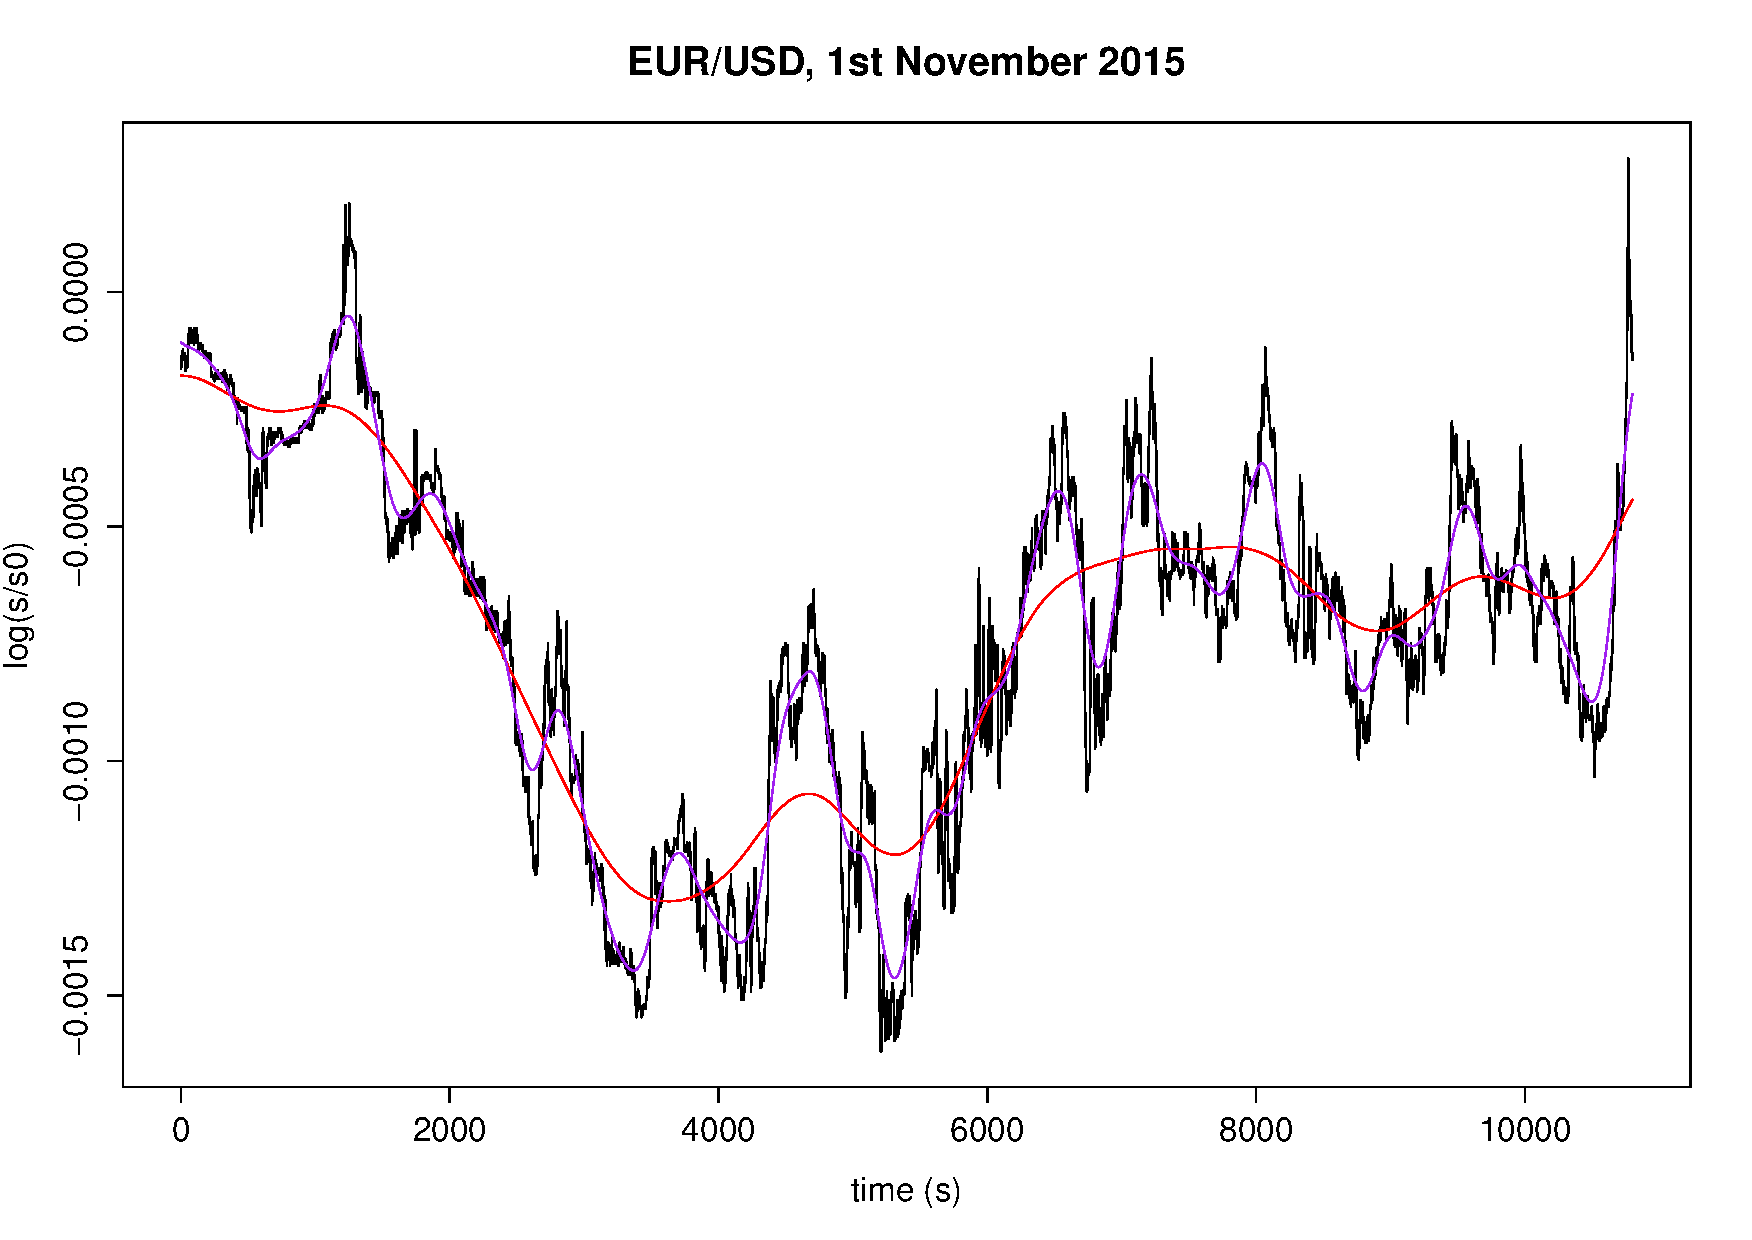
\includegraphics[width=0.7\textwidth]{figures/asset/ex_filtering}
\caption{\textbf{Exemple de la structure multi-scalaire du signal qui sert de base à la construction des signaux synthétiques | } Les \emph{log-prix} sont représentés sur environ 3h pour la journée du 1er novembre 2015 pour l'actif EUR/USD, ainsi que les tendances à 10min (violet) et à 30min.}
\label{fig:example_signal}
\end{figure}
%%%%%%%%%%%%%%%%%%%




%%%%%%%%%%%%%%%%%%%
\begin{figure}
\centering
% figure : effective correlations, with confidence intervals (bootstrap), for the 3 filtering scales. ; AND expected corrected corrs from derivation above.
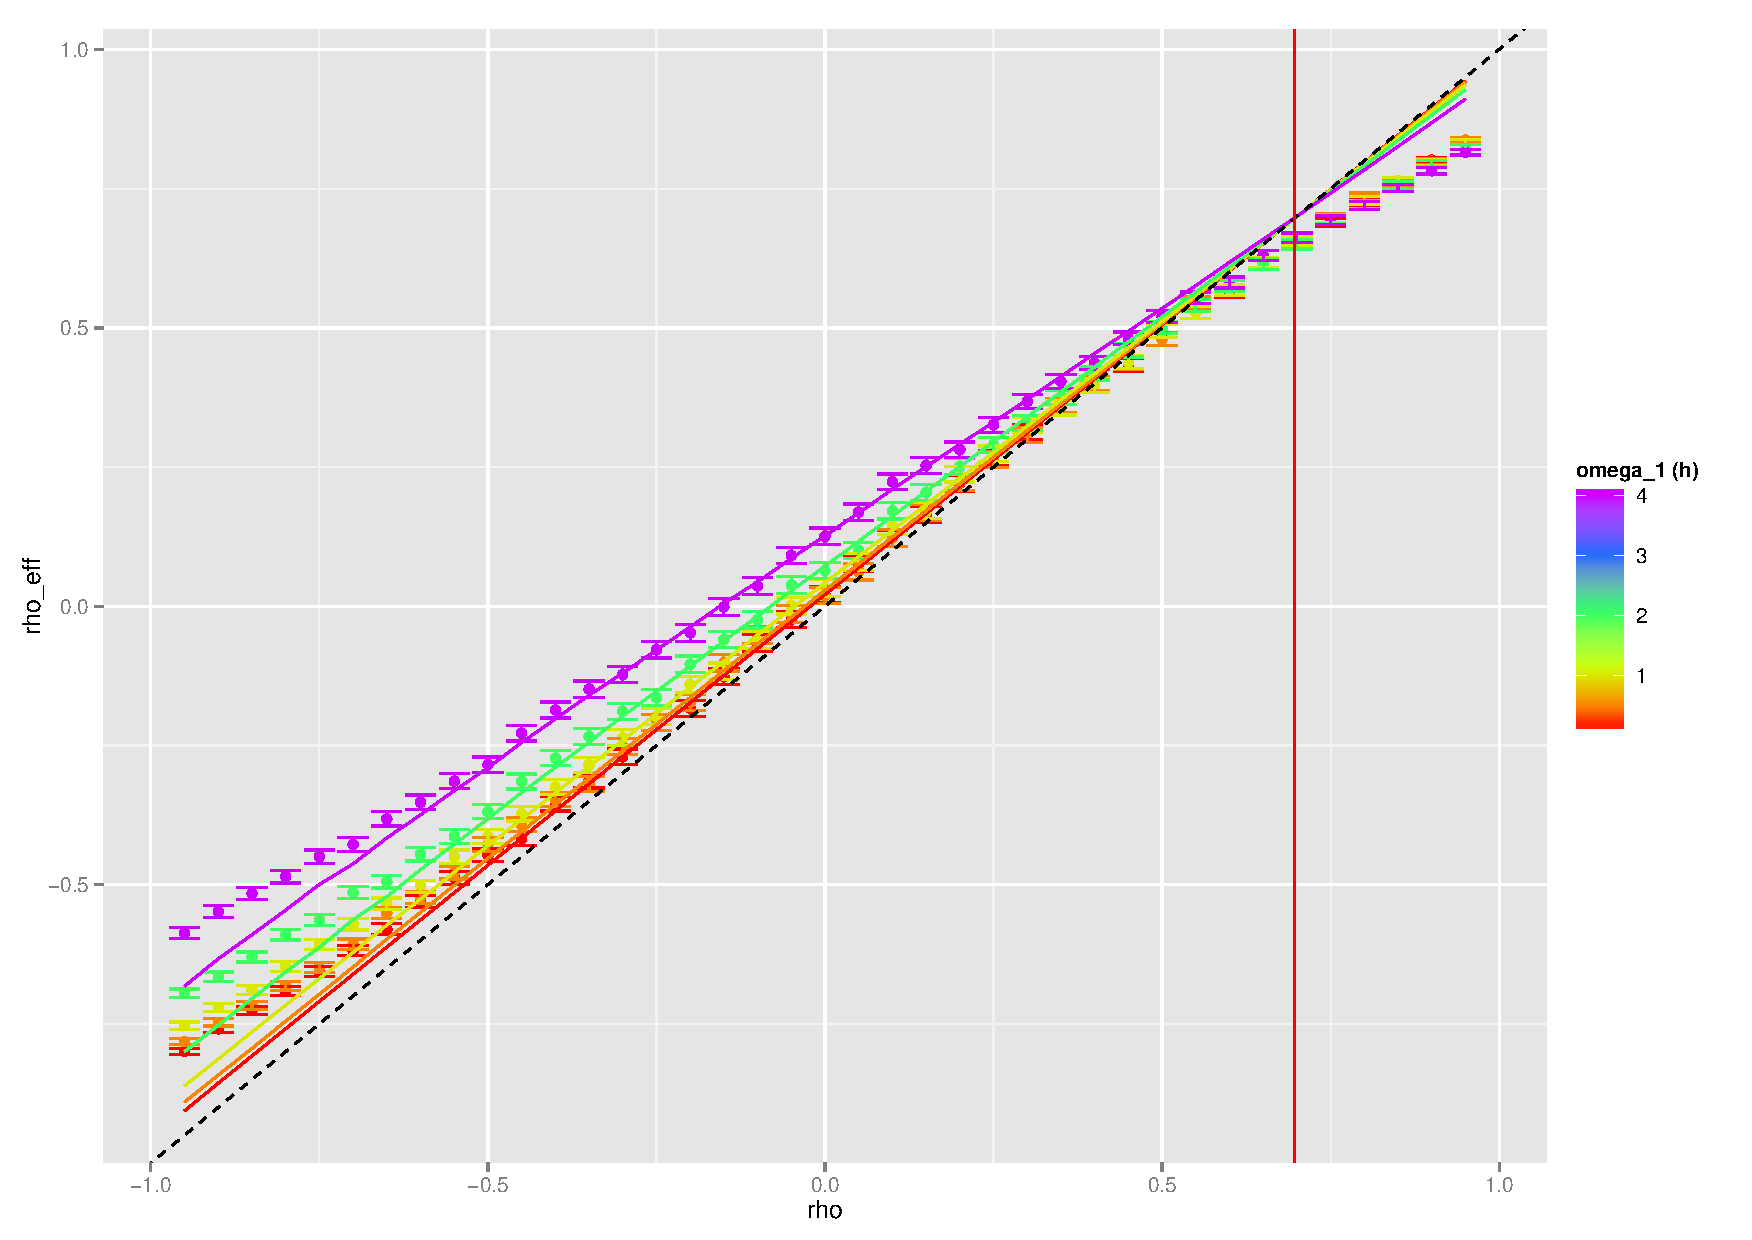
\includegraphics[width=0.7\textwidth]{figures/effectiveCorrs_withGoodTh_A4}
\caption{\textbf{Correlations effectives obtenues sur les données synthétiques | } Les points représentent les correlations estimées sur une génération d'un jeu de données synthétiques correspondant aux 6 mois de juin à novembre 2015 (barres d'erreurs obtenue par méthode de Fisher standard) ; l'échelle de couleur donne la fréquence de filtrage $\omega_1=10\textrm{min},30\textrm{min},1\textrm{h},2\textrm{h},4\textrm{h}$ ; les courbes sont les valeurs théoriques de $\rho_e$ obtenues par~\ref{eq:eff_corr} avec les volatilités estimées (diagonale en pointillés pour référence) ; l'abscisse de la ligne rouge est la valeur théorique telle que $\rho = \rho_e$ avec les valeurs moyennes de $\varepsilon_i$ sur l'ensemble des points. On observe dans les fortes correlations une déviation des valeurs corrigées, qui peut être dû aux hypothèses d'indépendance ou d'espérance nulle non vérifiées. La dissymétrie de la courbe est causée par la forte valeur positive de $\rho_0 \simeq 0.71$.}
\label{fig:effective_corrs}
\end{figure}
%%%%%%%%%%%%%%%%%%%


%%%%%%%%%%%%%%%%%%%
\begin{figure}
% figure : performance of arma2 as a function of expected correlation.

\caption{}
\label{fig:model_perf}
\end{figure}
%%%%%%%%%%%%%%%%%%%





%%%%%%%%%%%%%%%%%%%%%%
\subsection{Application : données géographiques de densité et de réseaux}


%%%%%%%%%%%%%%%%%%%%%%
\subsubsection{Contexte}


En géographie, l'utilisation de données synthétiques est plus généralement axée vers l'utilisation de population synthétiques au sein de modèles basés agents (mobilité, modèles \emph{LUTI})~\cite{pritchard2009advances}. Il a récemment été proposé de contrôler systématiquement les effets de la configuration spatiale sur le comportement de modèles de simulation spatialisés~\cite{cottineau2015revisiting}, méthodologie pouvant être interprétée comme un contrôle par données statistiques spatiales. L'enjeu est de pouvoir alors distinguer effets propres dus à la dynamique intrinsèque du modèle, d'effet particuliers dus à la structure géographique du cas d'application. Celui-ci est crucial pour la validation des conclusions issues des pratiques de modélisation et simulation en géographie quantitative.


%%%%%%%%%%%%%%%%%%%%%%
\subsubsection{Formalisation}

Dans notre cas, nous proposons de générer des systèmes de villes représentés par une densité spatiale de population $d(\vec{x})$ et la donnée d'un réseau de transport $n(\vec{x})$, représenté de façon simplifiée, pour lesquels on serait capable de contrôler les correlations entre mesures morphologiques de la densité urbaine et caractéristiques du réseau. Nous proposons un couplage \emph{simple}


\paragraph{Modèle de densité}

L'utilisation d'un modèle $D$ type agrégation-diffusion~\cite{batty2006hierarchy} permet de générer une distribution discrete de densité. Dans \cite{raimbault2016calibration}, une généralisation de ce modèle est calibré pour des objectifs morphologiques (entropie, hiérarchie, auto-corrélation spatiale, distance moyenne) contre les valeurs réelles calculées sur l'ensemble des grilles de taille 50km extraites de la grille européenne de densité~\cite{eurostat}. Plus précisément, le modèle fonctionne de manière itérative de la façon suivante. Une grille initialement vide de côté $N$, est représentée par la données des populations $(P_i(t))_{1\leq i\leq N^2}$. A chaque pas de temps, jusqu'à ce que la population atteigne une valeur fixée $P_m$,
\begin{itemize}
\item la population totale $P(t)$ est augmentée d'un nombre fixé $N_G$ (taux de croissance), suivant un attachement préférentiel tel que $\Pb{P_i(t+1)=P_i(t)+1|P(t+1)=P(t)+1}=\frac{(P_i(t)/P(t))^{\alpha}}{\sum(P_i(t)/P(t))^{\alpha}}$
\item une diffusion d'une fraction $\beta$ de la population aux 4 plus proches voisins est effectuée $n_d$ fois
\end{itemize}

Les deux processus antagonistes de concentration et d'étalement urbain sont capturés par le modèle, ce qui permet de reproduire assez fidèlement un grand nombre de morphologies existantes.


\paragraph{Modèle de réseau}

D'autre part, on est capable de générer par un modèle $N$ un réseau de transport planaire à une échelle équivalente, étant donné une distribution de densité. La génération du réseau étant conditionnée à la donnée de la densité, les estimateurs des indicateurs de réseau seront conditionnels d'une part, et d'autre part les formes urbaines et du réseau devraient nécessairement être corrélées, les processus n'étant pas indépendants. La nature et la modularité de ces correlations selon la variation des paramètres des modèles restent à déterminer par l'exploration du modèle couplé.

La procédure de génération heuristique de réseau est la suivante :
\begin{enumerate}
\item Un nombre fixé $N_c$ de centres qui seront les premiers noeuds du réseau est distribué selon la distribution de densité, suivant une loi similaire à celle d'agrégation, i.e. la probabilité d'être distribué sur une case est $\frac{(P_i/P)^{\alpha}}{\sum (P_i/P)^{\alpha}}$. La population est ensuite répartie selon les zones de Voronoi des centres, un centre cumulant la population des cases dans son emprise.
\item Les centres sont connectés de façon déterministe par percolation entre plus proches clusters : tant que le réseau n'est pas connexe, les deux composantes connexes les plus proches au sens de la distance minimale entre chacun de leurs sommets sont connectées par le lien réalisant cette distance. On obtient alors un réseau arborescent.
\item Le réseau est alors modulé par ruptures de potentiels afin de se rapprocher de formes réelles. Plus précisément, un potentiel d'interaction gravitaire généralisé entre deux centres $i$ et $j$ est défini par
\[
V_{ij}(d) = \left[ (1 - k_h) + k_h \cdot \left( \frac{P_i P_j}{P^2} \right)^{\gamma} \right]\cdot \exp{\left( -\frac{d}{r_g (1 + d/d_0)} \right)}
\]

où $d$ peut être la distance euclidienne $d_{ij}=d(i,j)$ ou la distance par le réseau $d_N(i,j)$, $k_h \in [0,1]$ un poids permettant de changer le rôle des population dans le potentiel, $\gamma$ régissant la forme de la hiérarchie selon les valeurs des populations, $r_g$ distance caractéristique de décroissance et $d_0$ paramètre de forme.
\item Un nombre $K\cdot N_L$ de nouveaux liens potentiels est pris comme les couples ayant le plus grand potentiel pour la distance euclidienne ($K=5$ est fixé).
\item Parmi les liens potentiels, $N_L$ sont effectivement réalisés, qui sont ceux ayant le plus faible rapport $V_{ij}(d_N)/V_{ij}(d_{ij})$ : à cette étape seul l'écart entre distance euclidienne et distance par le réseau compte, ce rapport ne dépendant plus des populations et étant croissant en $d_N$ à $d_{ij}$ fixé.
\item Le réseau est planarisé par création de noeuds aux intersections éventuelles créées par les nouveaux liens.
\end{enumerate}


Notons que la construction du modèle de génération est heuristique, et que d'autres types de modèles comme un réseau biologique auto-généré~\cite{TeroAl10}, une génération par contraintes géométriques locales~\cite{barthelemy2008modeling} ou un modèle de percolation plus complexe que celui utilisé, peuvent le remplacer. Ainsi, dans le cadre d'une architecture modulaire où le choix entre différentes implémentations d'une brique fonctionnelle peut être vue comme méta-paramètre~\cite{cottineau2015incremental}, on pourrait choisir la fonction de génération adaptée à un besoin donné (par exemple proximité à des données réelles, contraintes sur les relations entre indicateurs de sortie, variété de formes générées, etc.).


\paragraph{Espace des paramètres}

L'espace des paramètres du modèle couplé\footnote{Le couplage faible permet de limiter le nombre total de paramètres puisqu'un couplage fort incluant des boucles de retroaction comprendrait nécessairement des paramètres supplémentaires pour régler la forme et l'intensité de celles-ci. Pour espérer le diminuer, il faudrait concevoir un modèle intégré, ce qui est différent d'un couplage fort dans le sens où il n'est pas possible de figer l'un des sous-systèmes pour obtenir un modèle de l'autre correspondant au modèle non-couplé.} est constitué des paramètres de génération de densité $\vec{\alpha}_D = (P_m/N_G , \alpha,\beta , n_d)$ (on s'intéresse pour simplifier au rapport entre population et taux de croissance, i.e. le nombre d'étapes nécessaires pour générer) et des paramètres de génération de réseau $\vec{\alpha}_N=(N_C,k_h,\gamma , r_g , d_0)$. On notera $\vec{\alpha} = (\vec{\alpha}_D,\vec{\alpha}_N)$.

\paragraph{Indicateurs}

On quantifie la forme urbaine et la forme du réseau, dans le but de moduler la corrélation entre ces indicateurs. La forme est définie par un vecteur $\vec{M}=(r,\bar{d},\varepsilon,a)$ donnant auto-corrélation spatiale (indice de Moran), distance moyenne, entropie, hiérarchie (voir~\cite{le2015forme} pour une définition précise de ces indicateurs). Les mesures de la forme du réseau $\vec{G} = (\bar{c},\bar{l},\bar{s},\delta)$ sont, avec le réseau noté $(V,E)$,
\begin{itemize}
\item Centralité moyenne $\bar{c}$, définie comme la moyenne de la \emph{betweeness-centrality} (normalisée dans $[0,1]$) sur l'ensemble des liens.
\item Longueur moyenne des chemins $\bar{l}$ définie par $\frac{1}{d_m}\frac{2}{|V|\cdot (|V|-1)}\sum_{i<j}d_N(i,j)$ avec $d_m$ distance de normalisation prise ici comme la diagonale du monde $d_m=\sqrt{2}N$.
\item Vitesse moyenne~\cite{banos2012towards}, qui correspond à la performance du réseau par rapport au trajet à vol d'oiseau, définie par $\bar{s} = \frac{2}{|V|\cdot (|V|-1)}\sum_{i<j}{\frac{d_{ij}}{d_N(i,j)}}$.
\item Diamètre du réseau $\delta = \max_{ij}d_N(i,j)$
\end{itemize}

\paragraph{Covariance et correlation}

On s'intéressera à la matrice de covariance croisée $\Covb{\vec{M}}{\vec{G}}$ entre densité et réseau, estimée sur un jeu de $n$ réalisations à paramètres fixés $(\vec{M}\left[D(\vec{\alpha})\right],\vec{G}\left[N(\vec{\alpha})\right])_{1\leq i\leq n}$ par l'estimateur standard non-biaisé. On prend comme correlation associée la correlation de Pearson estimée de la même façon.



%%%%%%%%%%%%%%%%%%%%%%
\subsubsection{Implémentation}

Le couplage des modèles génératifs est effectué à la fois au niveau formel et au niveau opérationnel, c'est à dire qu'on fait interagir des implémentations indépendantes. Pour cela, le logiciel OpenMole~\cite{reuillon2013openmole} utilisé pour l'exploration intensive, offre le cadre idéal de par son langage modulaire permettant de construire des \emph{workflows} par composition de tâches à loisir et de les brancher sur divers plans d'expérience et sorties. Pour des raisons opérationnelles, le modèle de densité est implémenté en langage \texttt{scala} comme un \texttt{plugin} d'OpenMole, tandis que la génération de réseau est implémentée en langage basé-agent \texttt{NetLogo}~\cite{wilensky1999netlogo}, ce qui facilite l'exploration interactive et construction heuristique interactive. Le code source est disponible pour reproductibilité sur le dépôt du projet\footnote{à l'adresse \texttt{https://github.com/JusteRaimbault/CityNetwork/tree/master/Models/Synthetic}}.



%%%%%%%%%%%%%%%%%%%%%%
\subsubsection{Résultats}

L'étude du modèle de densité seul est développée dans~\cite{raimbault2016calibration}. Il est notamment calibré sur les données de la grille européenne de densité, sur des zones de 50km de côté et de résolution 500m pour lesquelles les valeurs réelles des indicateurs ont été calculées pour l'ensemble de l'Europe. D'autre part, une exploration brutale du modèle permet d'estimer l'ensemble des sorties possibles dans des bornes raisonnables pour les paramètres (grossièrement $\alpha \in [0.5,2],N_G\in [500,3000], P_m \in [10^4,10^5],\beta\in [0,0.2], n_d \in \{ 1, \ldots , 4\}$). La réduction à un plan de l'espace des objectif par une Analyse en Composantes Principales (variance expliquée à deux composantes $\simeq 80\%$) permet d'isoler un nuage de points de sorties recouvrant assez fidèlement le nuage des points réels, ce qui veut dire que le modèle est capable de reproduire morphologiquement l'ensemble des configurations existantes.


% NOT NEEDED - TOO MUCH INFORMATION - ?
%%%%%%%%%%%%%%%%
%\begin{figure}
% figure : density example, exploration and calibration ?
%\end{figure}
%%%%%%%%%%%%%%%%

A densité donnée, l'exploration de l'espace des paramètres du modèle de réseau suggèrent une assez bonne flexibilité sur des indicateurs globaux $\vec{G}$, ainsi que de bonnes propriétés de convergence. Pour une étude du comportement précis, voir l'appendice donnant les regressions traduisant le comportement du modèle couplé. Dans le but d'illustrer la méthode de génération de données synthétiques, l'exploration a été orientée vers l'étude des correlations.

Etant donné la grande dimension relative de l'espace des paramètres, une exploration par grille exhaustive est impossible. On utilise un plan d'expérience par criblage (hypercube latin), avec les bornes indiquées ci-dessus pour $\vec{\alpha}_D$ et pour $\vec{\alpha}_N$, on a $N_C \in [50,120], r_g \in [1,100] , d_0 \in [0.1,10] , k_h \in [0,1] , \gamma \in [0.1,4],N_L\in [4,20]$. Concernant le nombre de réplications du modèle pour chaque valeur des paramètres, moins de 50 sont nécessaires pour obtenir sur les indicateurs des intervalles de confiance à 95\% de taille inférieure aux déviations standard. Pour les correlations, une centaine donne des IC (obtenus par méthode de Fisher) de taille moyenne 0.4, on fixe donc $n=80$ pour l'expérience. La figure~\ref{fig:densnwcor} donne le détail des résultats de l'exploration. On retiendra les résultats marquants suivants au regard de la génération de données synthétiques corrélées :
\begin{itemize}
\item les distributions empiriques des coefficients de correlations entre indicateurs de forme et indicateurs de réseaux ne sont pas simples, pouvant être bimodales (par exemple $\rho_{46}=\rho[r,\bar{l}]$ entre l'index de Moran et le chemin moyen).
\item On arrive à générer un assez haut niveau de correlation pour l'ensemble des indicateurs, la correlation absolue maximale variant entre 0.6 et 0.9 ; l'amplitude varie quant à elle entre 0.9 et 1.6, ce qui permet un large spectre de valeurs. 
\item les points les plus corrélés en moyenne sont également ceux les plus proches des données réelles, ce qui confirme l'intuition d'une forte interdépendance en réalité.
\end{itemize}



\subsubsection{Extensions possibles}

On pourra éventuellement appliquer des algorithmes plus fins d'exploration pour atteindre des configurations exceptionelles réalisant un niveau de corrélation voulu~\cite{10.1371/journal.pone.0138212}. Les indicateurs globaux devraient ainsi être corrélés à un niveau contrôlé, tandis que les densités et réseaux restent cohérents dans l'espace de par la forme du réseau, conditionnelle à la distribution de densité. Les applications géographiques potentielles de cette implémentation de la méthode incluent le contrôle statistique de l'effet des corrélations entre ville et réseaux sur des modèles de simulation spatiaux par exemple.


 ainsi que la calibration contre les mesures réelles calculées sur l'ensemble de l'Europe sur des zones identiques au modèle de densité, via les données de réseau routier d'OpenStreetMap. La connaissance très fine ainsi obtenue du comportement de $N$ (distribution statistiques sur une grille fine de l'espace des paramètres à trois dimensions), devrait permettre, étant donné une population de configuration de densités $\tilde{D}$, de déterminer via $N^{<-1>}$ une population de réseau $\tilde{N}$ telle que $\Covb{M}{G}$ a une structure fixée (via la détermination de la valeur des paramètres à utiliser pour chaque individu de $\tilde{D}$). 


% également calib sur forme du réseau ?


%%%%%%%%%%%%%%
\begin{figure}

\begin{subfigure}[t]{0.35\linewidth}
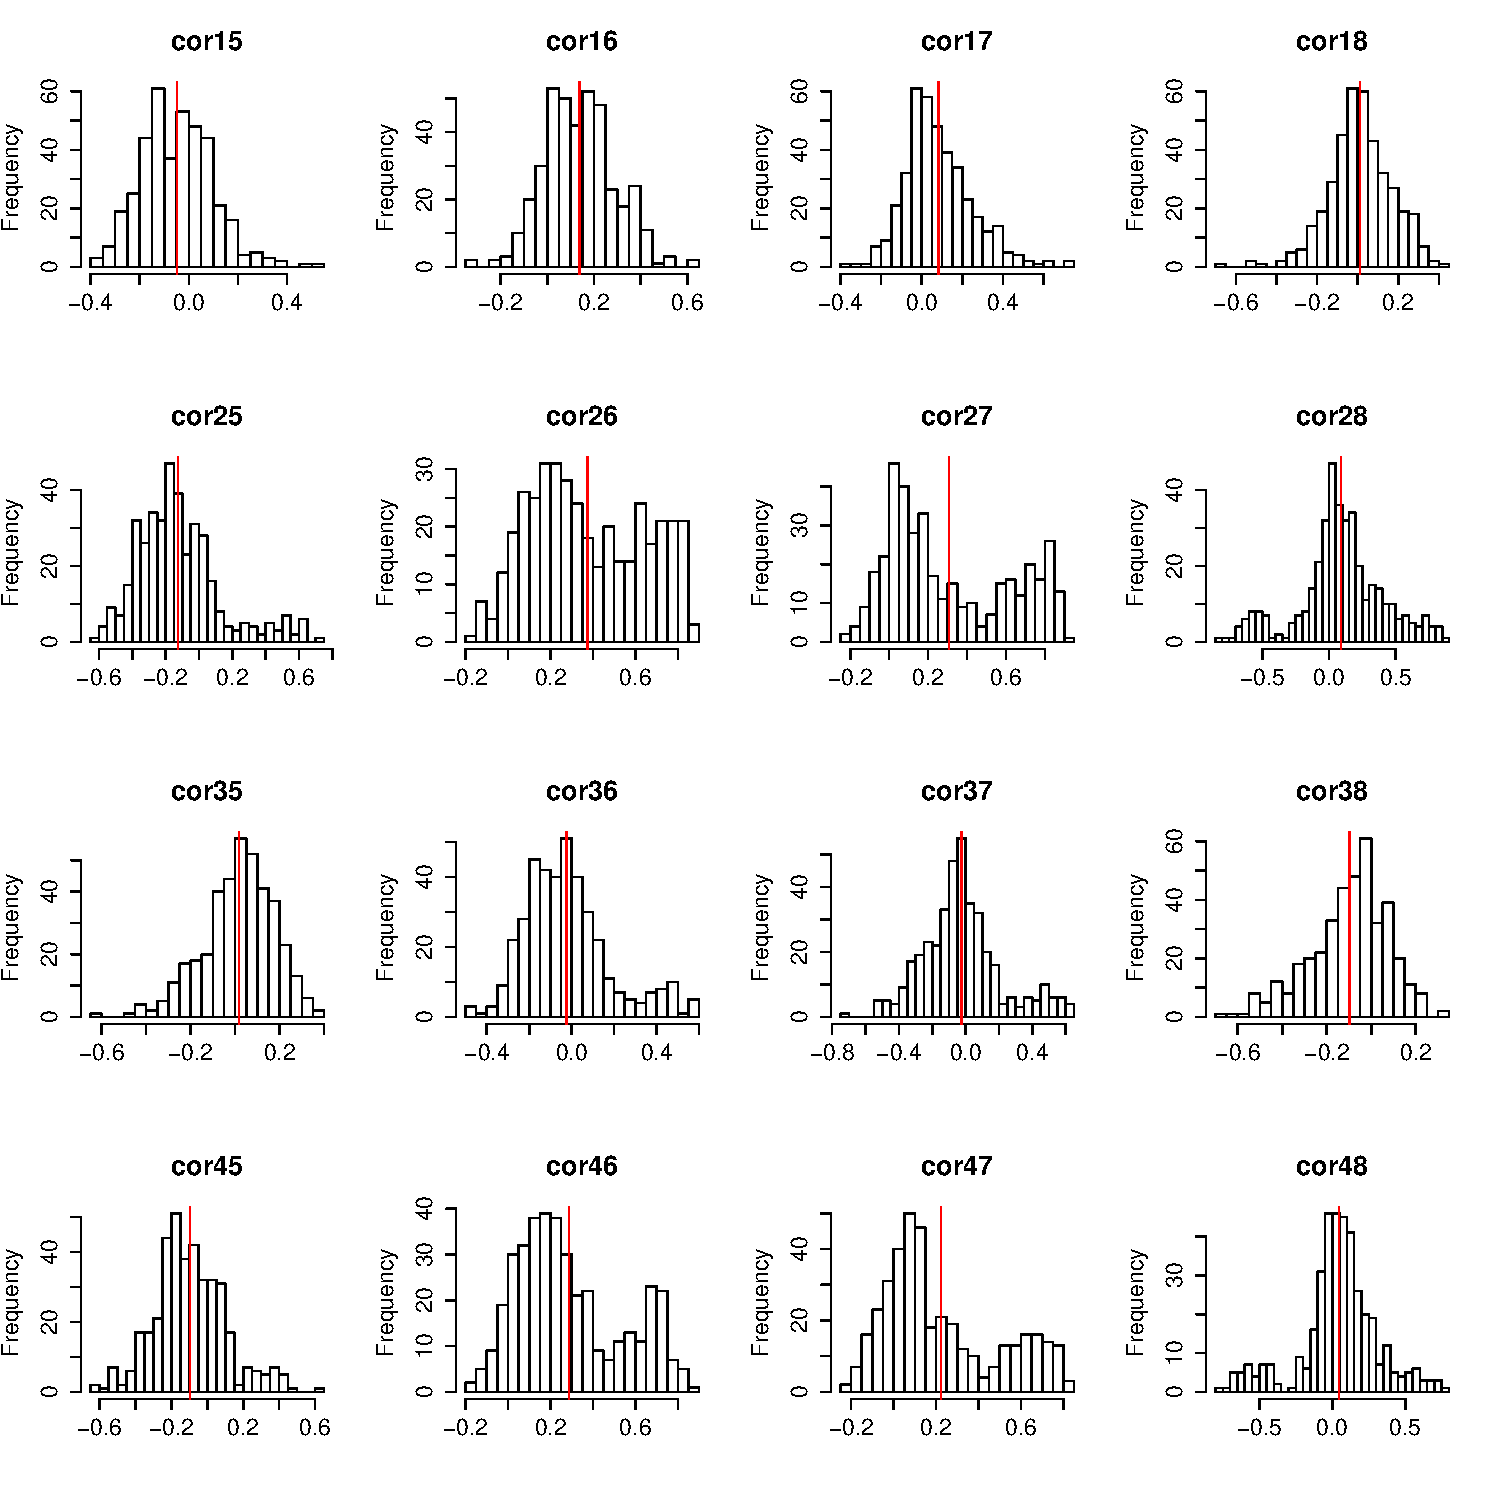
\includegraphics[width=\textwidth]{figures/hist_crossCorMat_breaks30}
\caption{}
\end{subfigure}
\begin{subfigure}[t]{0.23\linewidth}
\vspace{-6.5cm}
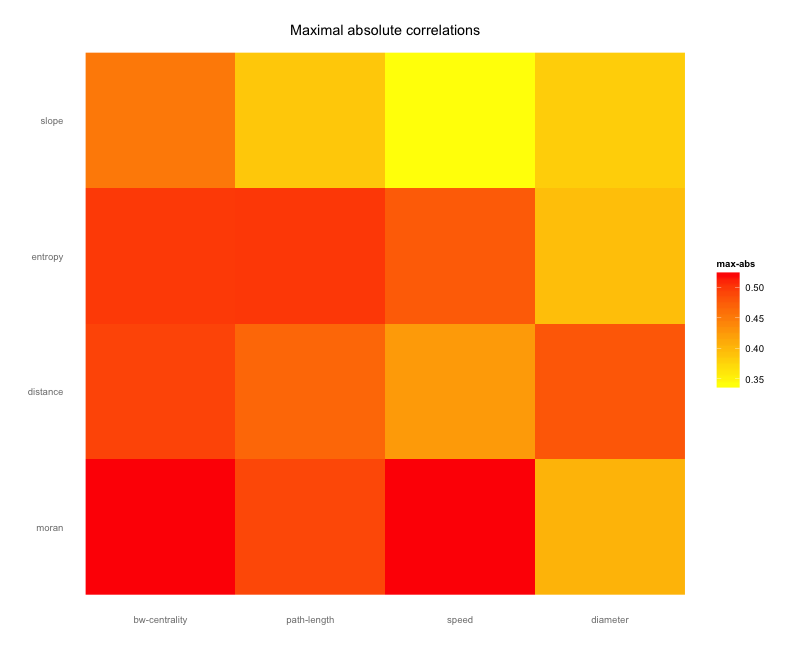
\includegraphics[width=\textwidth]{figures/heatmap_maxAbsCor}\\
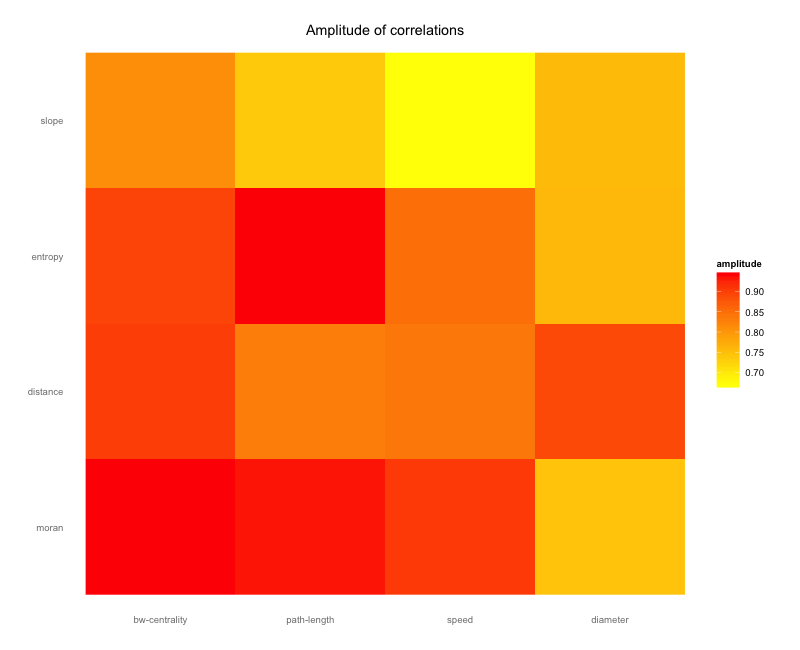
\includegraphics[width=\textwidth]{figures/heatmap_amplCor}
\caption{}
\end{subfigure}
\begin{subfigure}[t]{0.4\linewidth}
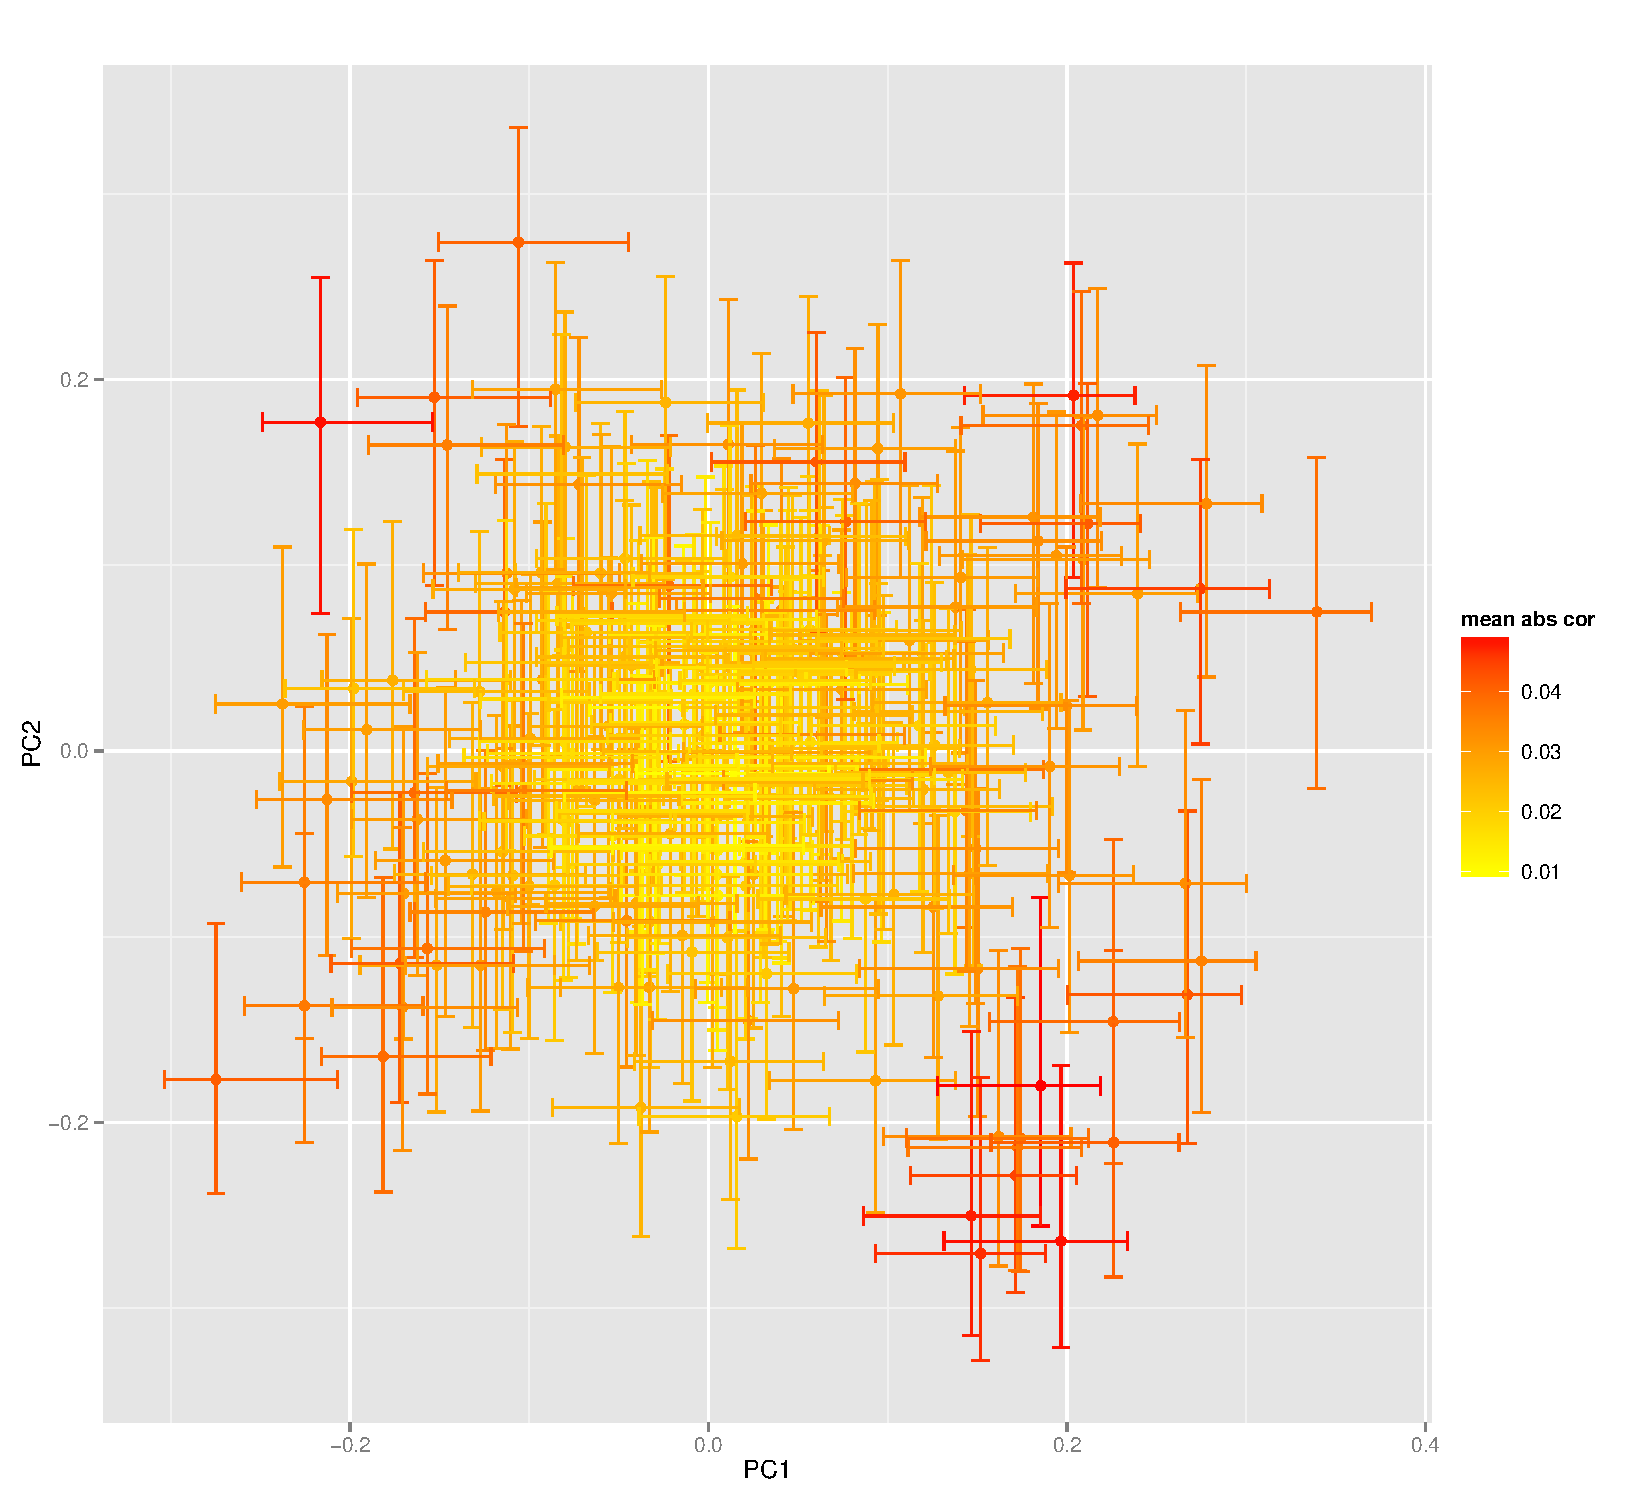
\includegraphics[width=\textwidth]{figures/pca_meanAbsCor_errorBars}
\caption{}
\end{subfigure}\\
\begin{subfigure}[t]{0.54\linewidth}
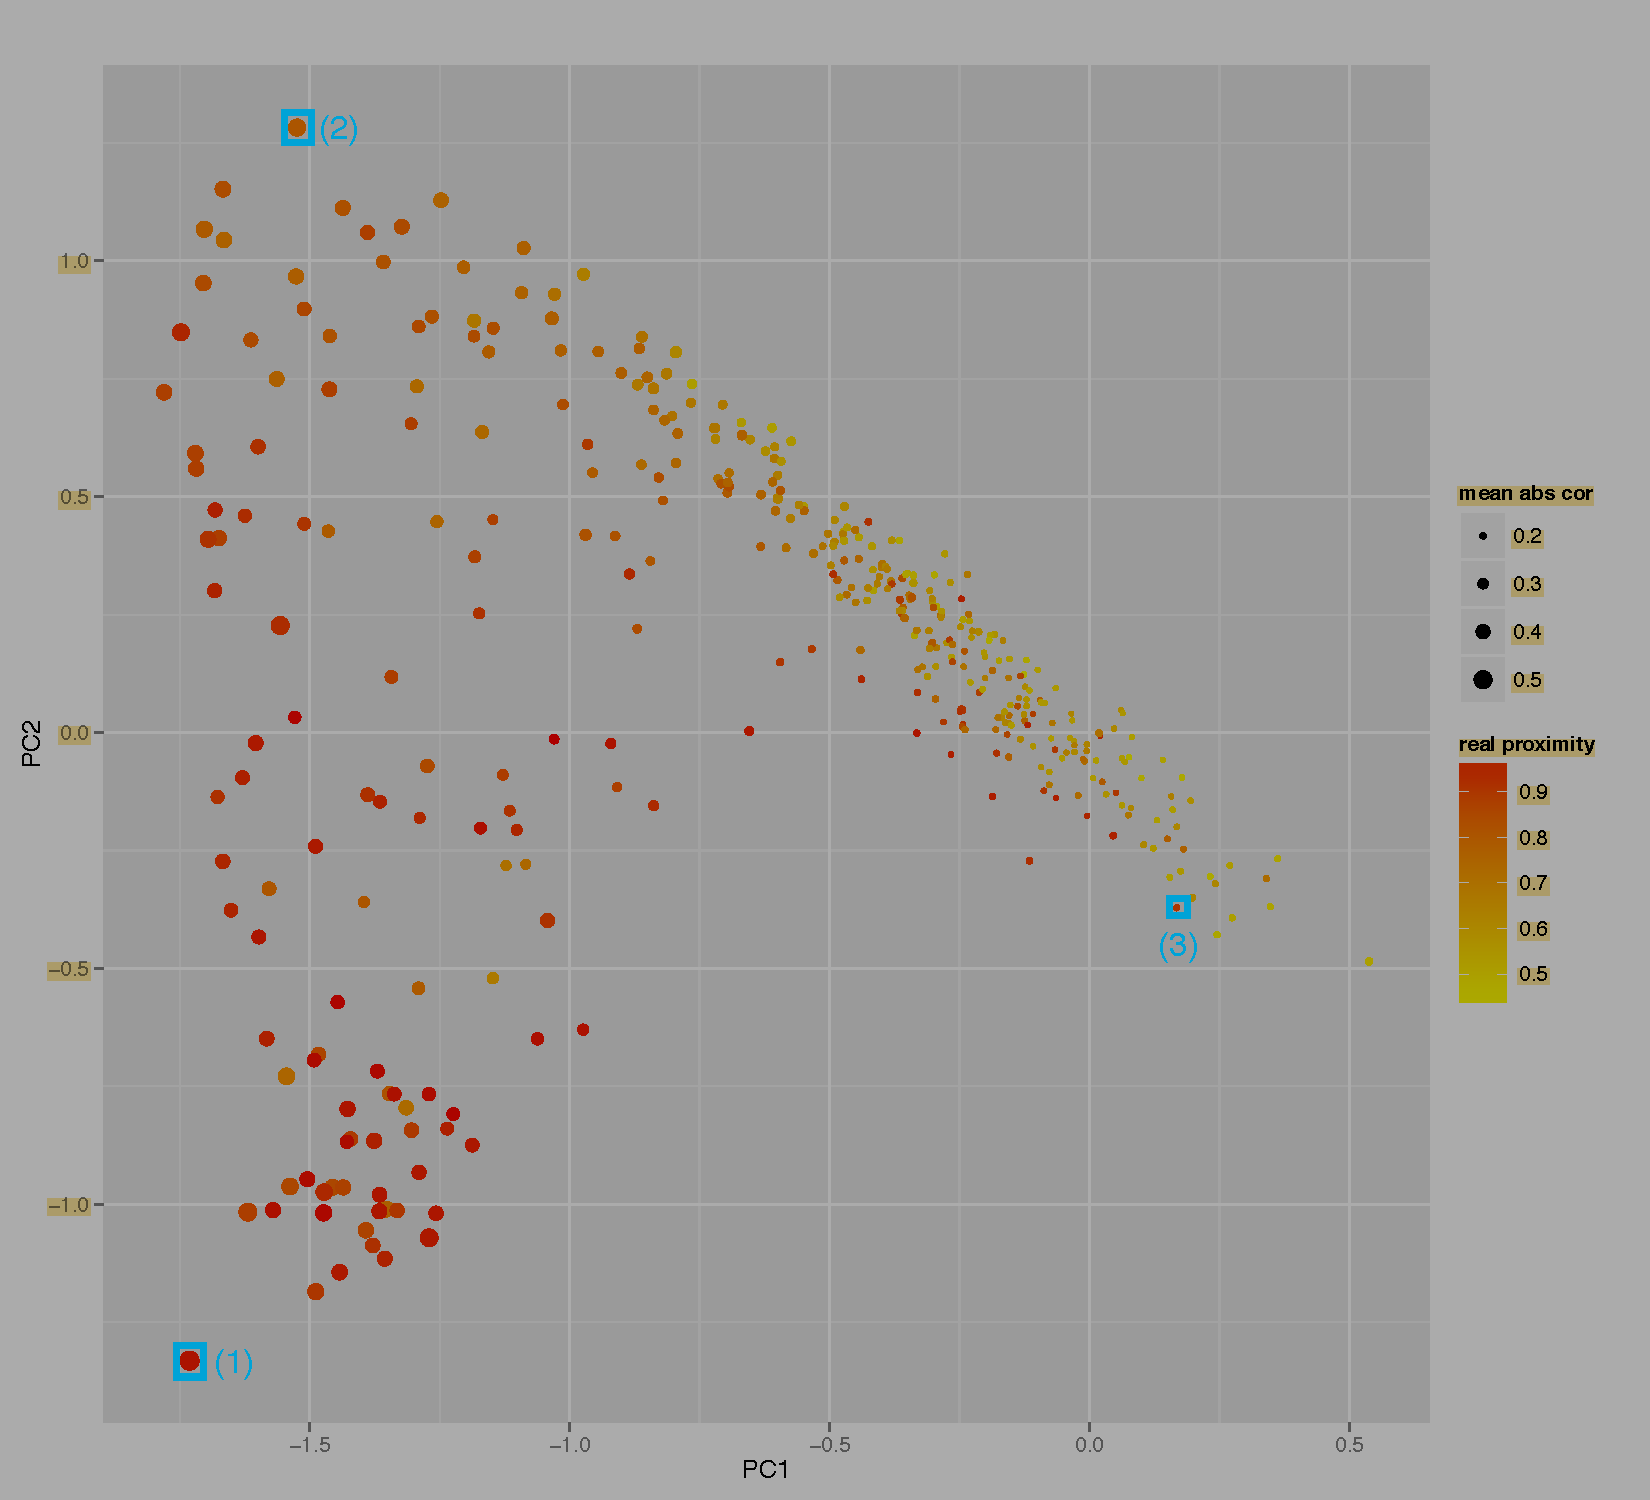
\includegraphics[width=\textwidth]{figures/pca_realDistCol_meanAbsCorSize_withSpecificPoints}
\caption{}
\end{subfigure}
\begin{subfigure}[t]{0.45\linewidth}
\vspace{-8.3cm}
   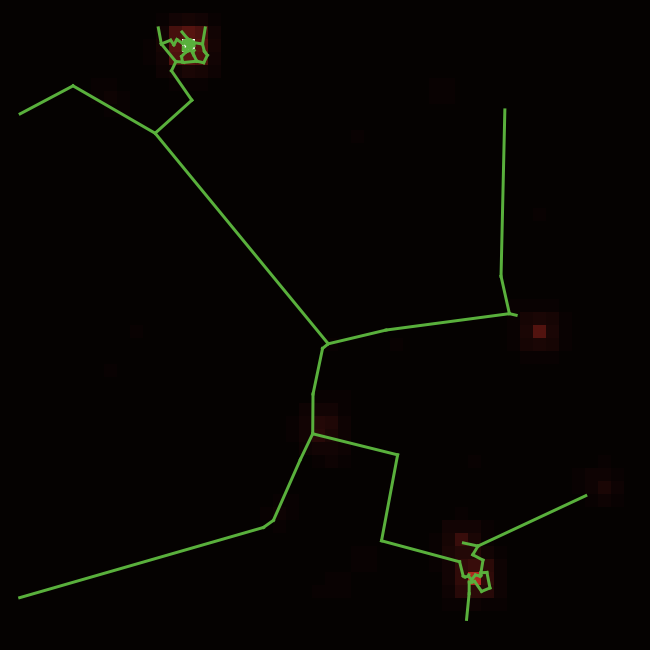
\includegraphics[width=0.49\textwidth]{figures/configs/1_param71861_seed0}
   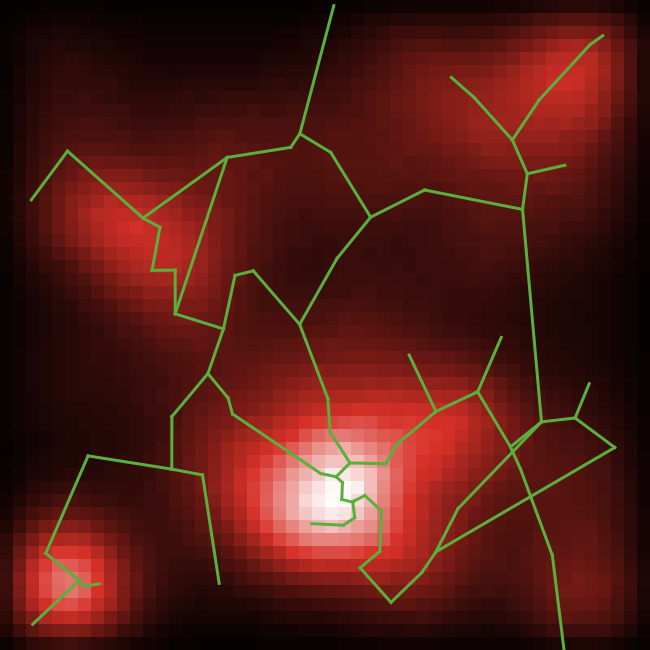
\includegraphics[width=0.49\textwidth]{figures/configs/2_param71913_seed10}\\
   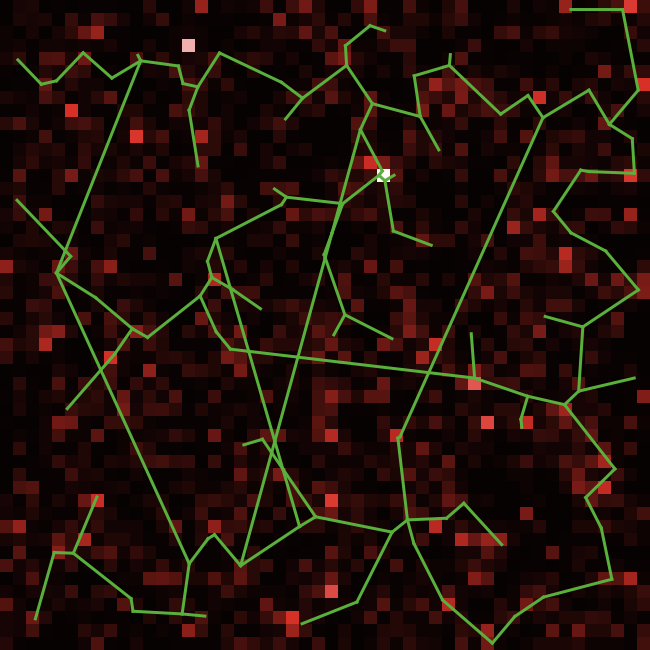
\includegraphics[width=0.49\textwidth]{figures/configs/3_param71918_seed0}
   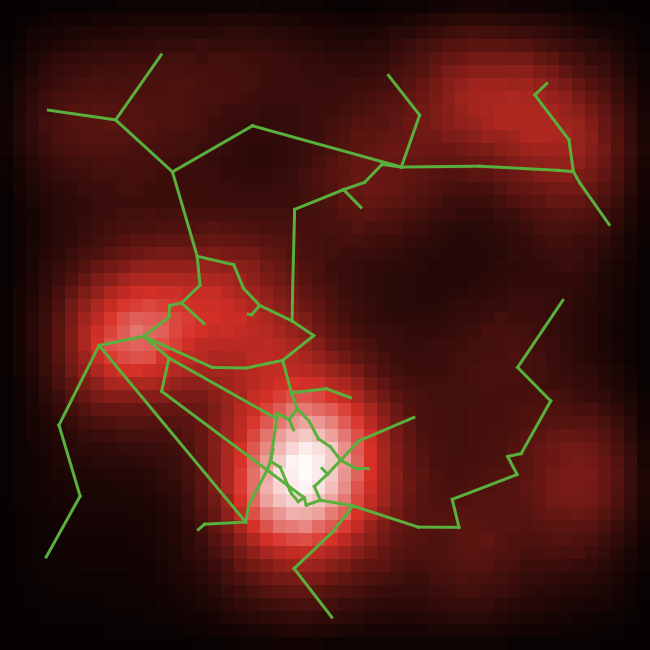
\includegraphics[width=0.49\textwidth]{figures/configs/4_param71945_seed0}
   \caption{}
\end{subfigure}

\caption{\small\textbf{Exploration de l'espace des corrélations entre forme urbaine et réseau | } \textbf{(a)} Distribution des correlations croisées entre les vecteurs $\vec{M}$ des indicateurs morphologiques (dans l'ordre index de moran, distance moyenne, entropie, hiérarchie) et $\vec{N}$ des mesures de réseau (centralité, longueur moyenne, vitesse, diamètre). \textbf{(b)} Amplitude des corrélations, définie comme $a_{ij}=\max_k{\rho_{ij}^{(k)}}-\min_k{\rho_{ij}^{(k)}}$, et correlation absolue maximale, $c_{ij}=\max_k\left| \right|$. \textbf{(c)} Représentation des matrices dans un plan principal obtenu par Analyse en Composantes Principales sur la population des matrices (variances cumulées: PC1=38\%, PC2=68\%). Les barres d'erreur sont calculées initialement par des intervalles de confiance à 95\% sur chaque élément de la matrice (par une méthode de Fisher asymptotique standard), puis les bornes supérieures sont prises dans le plan principal. L'échelle de couleur donne la correlation absolue moyenne sur l'ensemble des variables. \textbf{(d)} }
\label{fig:densnwcor}
\end{figure}
%%%%%%%%%%%%%%



%%%%%%%%%%%%%%
\begin{table}
%regression analysis of param influence on correlations

\end{table}
%%%%%%%%%%%%%%





%%%%%%%%%%%%%%%%%%%%%%
\section{Discussion}
%%%%%%%%%%%%%%%%%%%%%%


%%%%%%%%%%%%%%%%%%%%%%
\subsection{Domaines potentiels d'application}

% ideas of other fields where the generation can happen.



%%%%%%%%%%%%%%%%%%%%%%
\subsection{Positionnement}

% données hybrides au centre de la démarche d'exploration de modèle, analyse de sensitivité etc.






%%%%%%%%%%%%%%%%%%%%%%
\section{Conclusion}
%%%%%%%%%%%%%%%%%%%%%%


On a ainsi proposé une méthode abstraite de génération de données synthétiques corrélées à un niveau contrôlé. Son implémentation partielle dans deux domaines très différents montre sa flexibilité et l'éventail des applications potentielles. De manière générale, il est essentiel de généraliser de telles pratiques de validation systématique de modèles par étude statistique, en particulier pour les modèles agents pour lesquels la question de la validation reste encore relativement ouverte.






\newpage


%%%%%%%%%%%%%%%%%%%%
%% Biblio
%%%%%%%%%%%%%%%%%%%%
\footnotesize

\bibliographystyle{apalike}
\bibliography{/Users/Juste/Documents/ComplexSystems/CityNetwork/Biblio/Bibtex/CityNetwork,biblio/biblio}





\newpage

%%%%%%%%%%%%%%%%%%%%
\section*{Appendice : Comportement du modèle couplé}



\subsection*{Indicateurs}

\begin{center}


\begin{tabular}{|c|c|c|c|c| }
 \hline
&BW&Pathlength&relspeed&diameter\\\hline
R2&0.6098&0.638 &0.7049 &0.5855\\\hline
(Intercept)&2.106e-01$\pm$ 4.728e-03 (***)&1.0939160$\pm$ 0.0514692 (***)&6.211e-01$\pm$ 9.722e-03 (***)&2.4956084$\pm$ 0.1172324 (***)\\
$\alpha$&-1.127e-02$\pm$ 2.012e-03 (***)&-0.5305835$\pm$ 0.0219066 (***)&8.469e-02$\pm$ 4.138e-03 (***)&-1.0366776$\pm$ 0.0498972 (***)\\
$\beta$&9.430e-03$\pm$ 6.803e-03 ()&0.1738349$\pm$ 0.0740571 (*)&-6.516e-02$\pm$ 1.399e-02 (***)&0.2937746$\pm$ 0.1686813 (.)\\
$n_d$&6.786e-04$\pm$ 6.534e-04 ()&0.0048631$\pm$ 0.0071129 ()&-4.046e-03$\pm$ 1.344e-03 (**)&0.0003039$\pm$ 0.0162012 ()\\
$N_C$&-3.005e-04$\pm$ 2.887e-05 (***)&0.0012026$\pm$ 0.0003143 (***)&-1.214e-03$\pm$ 5.937e-05 (***)&0.0040004$\pm$ 0.0007159 (***)\\
$N_G$&4.800e-02$\pm$ 1.348e-02 (***)&1.4969583$\pm$ 0.1467356 (***)&-1.400e-01$\pm$ 2.772e-02 (***)&3.3021779$\pm$ 0.3342227 (***)\\
$\gamma$&4.615e-03$\pm$ 4.997e-04 (***)&0.0132129$\pm$ 0.0054394 (*)&-7.990e-03$\pm$ 1.027e-03 (***)&0.0389784$\pm$ 0.0123895 (**)\\
$d_0$&2.743e-04$\pm$ 1.971e-04 ()&-0.0029289$\pm$ 0.0021453 ()&-5.688e-04$\pm$ 4.052e-04 ()&-0.0075661$\pm$ 0.0048863 ()\\
$r_g$&-2.726e-05$\pm$ 2.038e-05 ()&0.0001532$\pm$ 0.0002219 ()&5.329e-05$\pm$ 4.191e-05 ()&0.0002358$\pm$ 0.0005054 ()\\
$k_h$&-1.035e-02$\pm$ 1.952e-03 (***)&-0.0954905$\pm$ 0.0212503 (***)&1.992e-02$\pm$ 4.014e-03 (***)&-0.2271416$\pm$ 0.0484021 (***)\\
$N_L$&-2.390e-03$\pm$ 1.243e-04 (***)&-0.0021779$\pm$ 0.0013533 ()&1.287e-03$\pm$ 2.556e-04 (***)&-0.0044759$\pm$ 0.0030824 ()\\

 \hline
\end{tabular}

\bigskip

\hspace{-0.4cm}

\begin{tabular}{|c|c|c|c|c| }
 \hline
&moran&distance&entropy&slope\\\hline
R2&0.7762&0.4753&0.5516&0.6587\\\hline
(Intercept)&1.106e-02$\pm$ 1.348e-02 ()&1.158e+00$\pm$ 3.862e-02 (***)&1.135e+00$\pm$ 3.024e-02 (***)&0.0839654$\pm$ 0.0706085 ()\\
$\alpha$&-1.631e-02$\pm$ 5.739e-03 (**)&-2.549e-01$\pm$ 1.644e-02 (***)&-2.396e-01$\pm$ 1.287e-02 (***)&-0.7543377$\pm$ 0.0300528 (***)\\
$\beta$&5.009e-01$\pm$ 1.940e-02 (***)&-2.497e-02$\pm$ 5.557e-02 ()&4.580e-01$\pm$ 4.351e-02 (***)&1.0974897$\pm$ 0.1015959 (***)\\
$n_d$&2.850e-02$\pm$ 1.863e-03 (***)&-1.069e-02$\pm$ 5.337e-03 (*)&1.630e-02$\pm$ 4.179e-03 (***)&0.0322148$\pm$ 0.0097579 (**)\\
$N_C$&-8.494e-05$\pm$ 8.234e-05 ()&-5.408e-05$\pm$ 2.358e-04 ()&-5.802e-05$\pm$ 1.847e-04 ()&0.0001797$\pm$ 0.0004312 ()\\
$N_G$&-7.710e-01$\pm$ 3.844e-02 (***)&1.222e+00$\pm$ 1.101e-01 (***)&4.276e-01$\pm$ 8.622e-02 (***)&1.0692012$\pm$ 0.2013007 (***)\\
$\gamma$&6.214e-04$\pm$ 1.425e-03 ()&2.219e-03$\pm$ 4.081e-03 ()&2.026e-03$\pm$ 3.196e-03 ()&-0.0015095$\pm$ 0.0074621 ()\\
$d_0$&2.457e-04$\pm$ 5.620e-04 ()&-3.896e-03$\pm$ 1.610e-03 (*)&-2.459e-03$\pm$ 1.261e-03 (.)&-0.0046572$\pm$ 0.0029430 ()\\
$r_g$&4.413e-05$\pm$ 5.813e-05 ()&1.048e-04$\pm$ 1.665e-04 ()&1.069e-04$\pm$ 1.304e-04 ()&0.0003902$\pm$ 0.0003044 ()\\
$k_h$&6.379e-03$\pm$ 5.567e-03 ()&-5.308e-02$\pm$ 1.595e-02 (***)&-3.215e-02$\pm$ 1.249e-02 (*)&-0.0407186$\pm$ 0.0291524 ()\\
$N_L$&5.183e-04$\pm$ 3.545e-04 ()&-4.340e-04$\pm$ 1.015e-03 ()&8.870e-06$\pm$ 7.952e-04 ()&0.0003567$\pm$ 0.0018565 ()\\
 \hline
\end{tabular}


\end{center}


\vspace{1cm}


\subsection*{Correlations}

\subsubsection*{Auto-correlations}

\begin{center}

\begin{tabular}{|c|c|c|c| }
 \hline
&$\rho[r,\bar{d}]$&$\rho[r,e]$&$\rho[r,s]$\\\hline
R2&0.5774&0.5093&0.5483\\\hline
(Intercept)&1.226986$\pm$0.034715 (***)&-1.104021$\pm$0.039630 (***)&1.21541$\pm$0.04161 (***)\\
$\alpha$&-0.497699$\pm$0.021858 (***)&0.472135$\pm$0.024953 (***)&-0.55056$\pm$0.02620 (***)\\
$\beta$&0.334188$\pm$0.073967 (***)&-0.606526$\pm$0.084439 (***)&0.46942$\pm$0.08866 (***)\\
$n_d$&0.008372$\pm$0.007066 ()&-0.023801$\pm$0.008066 (**)&0.01310$\pm$0.00847 ()\\
$N_G$&0.665346$\pm$0.146472 (***)&-0.483421$\pm$0.167209 (**)&0.99527$\pm$0.17557 (***)\\
\hline
\end{tabular}

\bigskip

\begin{tabular}{|c|c|c|c| }
 \hline
&$\rho[\bar{d},e]$&$\rho[\bar{d},s]$&$\rho[e,s]$\\\hline
R2&0.5141&0.5383&0.5449\\\hline
(Intercept)&-1.67032$\pm$0.08598 (***)&1.043888$\pm$0.016697 (***)&-1.50417$\pm$0.07318 (***)\\
$\alpha$&1.04667$\pm$0.05414 (***)&-0.218800$\pm$0.010513 (***)&0.95046$\pm$0.04608 (***)\\
$\beta$&-0.91864$\pm$0.18320 (***)&0.153942$\pm$0.035577 (***)&-0.80453$\pm$0.15592 (***)\\
$n_d$&-0.04144$\pm$0.01750 (*)&0.007833$\pm$0.003399 (*)&-0.03624$\pm$0.01489 (*)\\
$N_G$&-2.23787$\pm$0.36278 (***)&0.355478$\pm$0.070450 (***)&-2.00208$\pm$0.30875 (***)\\
 \hline
\end{tabular}



\end{center}



\subsubsection*{Correlations croisées}


\begin{center}

\begin{tabular}{|c|c|c|c|c| }
 \hline
&$\rho[r,\bar{c}]$&$\rho[r,\bar{l}]$&$\rho[r,\bar{s}]$&$\rho[r,\delta]$\\\hline
R2&0.08052&0.1734&0.174&0.1187\\\hline
(Intercept)&-0.0262848$\pm$0.0582459 ()&-1.830e-01$\pm$5.801e-02 (**)&-2.800e-01$\pm$6.381e-02 (***)&-0.0396938$\pm$0.0609953 ()\\
$\alpha$&0.0425576$\pm$0.0247910 (.)&2.239e-01$\pm$2.469e-02 (***)&2.369e-01$\pm$2.716e-02 (***)&-0.0546067$\pm$0.0259612 (*)\\
$\beta$&-0.3076801$\pm$0.0838078 (***)&2.970e-02$\pm$8.347e-02 ()&2.487e-02$\pm$9.182e-02 ()&0.4311665$\pm$0.0877639 (***)\\
$n_d$&-0.0225112$\pm$0.0080494 (**)&-2.231e-03$\pm$8.017e-03 ()&8.874e-03$\pm$8.819e-03 ()&0.0418159$\pm$0.0084294 (***)\\
$N_C$&0.0001178$\pm$0.0003557 ()&2.270e-04$\pm$3.542e-04 ()&3.001e-04$\pm$3.897e-04 ()&-0.0004806$\pm$0.0003725 ()\\
$N_G$&0.4455534$\pm$0.1660556 (**)&-5.238e-01$\pm$1.654e-01 (**)&-6.272e-01$\pm$1.819e-01 (***)&-0.2879462$\pm$0.1738941 (.)\\
$\gamma$&-0.0153085$\pm$0.0061556 (*)&4.880e-03$\pm$6.131e-03 ()&-3.259e-03$\pm$6.744e-03 ()&0.0076671$\pm$0.0064462 ()\\
$d_0$&0.0019859$\pm$0.0024277 ()&2.813e-03$\pm$2.418e-03 ()&-3.898e-05$\pm$2.660e-03 ()&0.0009132$\pm$0.0025423 ()\\
$r_g$&0.0001959$\pm$0.0002511 ()&5.983e-05$\pm$2.501e-04 ()&9.584e-05$\pm$2.751e-04 ()&-0.0001899$\pm$0.0002629 ()\\
$k_h$&0.0412129$\pm$0.0240482 (.)&2.120e-02$\pm$2.395e-02 ()&5.927e-02$\pm$2.635e-02 (*)&-0.0178174$\pm$0.0251834 ()\\
$N_L$&-0.0011826$\pm$0.0015315 ()&5.317e-05$\pm$1.525e-03 ()&7.111e-04$\pm$1.678e-03 ()&0.0006752$\pm$0.0016037 ()\\
\hline
\end{tabular}

\bigskip

\begin{tabular}{|c|c|c|c|c| }
 \hline
&$\rho[\bar{d},\bar{c}]$&$\rho[\bar{d},\bar{l}]$&$\rho[\bar{d},\bar{s}]$&$\rho[\bar{d},\delta]$\\\hline
R2&0.09957&0.726&0.6635&0.2736\\\hline
(Intercept)&-7.875e-03$\pm$1.000e-01 ()&-5.920e-01$\pm$5.909e-02 (***)&-0.8352368$\pm$0.0769938 (***)&-0.2136136$\pm$0.1134114 (.)\\
$\alpha$&1.143e-02$\pm$4.257e-02 ()&7.915e-01$\pm$2.515e-02 (***)&0.8797555$\pm$0.0327706 (***)&-0.0164318$\pm$0.0482709 ()\\
$\beta$&-6.376e-01$\pm$1.439e-01 (***)&-9.049e-02$\pm$8.502e-02 ()&0.0652982$\pm$0.1107835 ()&1.6099651$\pm$0.1631834 (***)\\
$n_d$&-4.068e-02$\pm$1.382e-02 (**)&-2.081e-03$\pm$8.166e-03 ()&0.0208547$\pm$0.0106403 (.)&0.0904758$\pm$0.0156732 (***)\\
$N_C$&3.524e-04$\pm$6.108e-04 ()&5.379e-05$\pm$3.608e-04 ()&0.0001255$\pm$0.0004702 ()&-0.0006020$\pm$0.0006926 ()\\
$N_G$&1.228e+00$\pm$2.851e-01 (***)&-1.668e+00$\pm$1.685e-01 (***)&-1.9878616$\pm$0.2195048 (***)&-1.1801054$\pm$0.3233292 (***)\\
$\gamma$&6.252e-03$\pm$1.057e-02 ()&-3.111e-03$\pm$6.244e-03 ()&-0.0036648$\pm$0.0081369 ()&0.0051939$\pm$0.0119857 ()\\
$d_0$&8.292e-04$\pm$4.169e-03 ()&2.533e-03$\pm$2.463e-03 ()&0.0003107$\pm$0.0032092 ()&-0.0029674$\pm$0.0047271 ()\\
$r_g$&4.879e-05$\pm$4.311e-04 ()&8.729e-05$\pm$2.547e-04 ()&-0.0001203$\pm$0.0003319 ()&0.0002683$\pm$0.0004889 ()\\
$k_h$&3.077e-02$\pm$4.129e-02 ()&2.040e-02$\pm$2.440e-02 ()&0.0403760$\pm$0.0317887 ()&-0.0958810$\pm$0.0468245 (*)\\
$N_L$&-5.190e-03$\pm$2.630e-03 (*)&1.228e-03$\pm$1.554e-03 ()&0.0017721$\pm$0.0020244 ()&0.0011045$\pm$0.0029819 ()\\
\hline
\end{tabular}

\bigskip

\begin{tabular}{|c|c|c|c|c| }
 \hline
&$\rho[e,\bar{c}]$&$\rho[e,\bar{l}]$&$\rho[e,\bar{s}]$&$\rho[e,\delta]$\\\hline
R2&0.08321&0.1137&0.04931&0.2212\\\hline
(Intercept)&1.229e-01$\pm$6.394e-02 (.)&-0.2235482$\pm$0.0796783 (**)&-1.069e-01$\pm$9.653e-02 ()&0.2851561$\pm$0.0647508 (***)\\
$\alpha$&-1.406e-01$\pm$2.721e-02 (***)&0.2003760$\pm$0.0339132 (***)&1.098e-01$\pm$4.109e-02 (**)&-0.2898858$\pm$0.0275597 (***)\\
$\beta$&3.474e-01$\pm$9.200e-02 (***)&-0.3847257$\pm$0.1146461 (***)&-4.382e-01$\pm$1.389e-01 (**)&0.1606966$\pm$0.0931675 (.)\\
$n_d$&1.386e-02$\pm$8.836e-03 ()&-0.0089831$\pm$0.0110113 ()&-2.277e-02$\pm$1.334e-02 (.)&-0.0058289$\pm$0.0089484 ()\\
$N_C$&-2.203e-04$\pm$3.904e-04 ()&0.0004494$\pm$0.0004866 ()&4.578e-04$\pm$5.895e-04 ()&0.0001080$\pm$0.0003954 ()\\
$N_G$&9.209e-02$\pm$1.823e-01 ()&-0.5779639$\pm$0.2271581 (*)&-4.211e-01$\pm$2.752e-01 ()&0.6379269$\pm$0.1846008 (***)\\
$\gamma$&6.198e-03$\pm$6.757e-03 ()&0.0024670$\pm$0.0084206 ()&3.531e-03$\pm$1.020e-02 ()&-0.0024161$\pm$0.0068431 ()\\
$d_0$&-1.465e-03$\pm$2.665e-03 ()&-0.0024864$\pm$0.0033211 ()&1.782e-03$\pm$4.023e-03 ()&-0.0017413$\pm$0.0026989 ()\\
$r_g$&-7.161e-05$\pm$2.756e-04 ()&-0.0002354$\pm$0.0003435 ()&-4.484e-04$\pm$4.161e-04 ()&-0.0001984$\pm$0.0002791 ()\\
$k_h$&-1.346e-02$\pm$2.640e-02 ()&0.0841865$\pm$0.0328970 (*)&9.604e-02$\pm$3.985e-02 (*)&-0.0061427$\pm$0.0267339 ()\\
$N_L$&9.124e-04$\pm$1.681e-03 ()&-0.0011866$\pm$0.0020950 ()&-8.891e-05$\pm$2.538e-03 ()&-0.0024391$\pm$0.0017025 ()\\
\hline
\end{tabular}

\bigskip

\begin{tabular}{|c|c|c|c|c| }
 \hline
&$\rho[s,\bar{c}]$&$\rho[s,\bar{l}]$&$\rho[s,\bar{s}]$&$\rho[s,\delta]$\\\hline
R2&0.05977&0.6849&0.5995&0.2071\\\hline
(Intercept)&6.096e-02$\pm$8.136e-02 ()&-0.5291554$\pm$0.0585027 (***)&-6.684e-01$\pm$7.185e-02 (***)&-0.1327534$\pm$0.1006121 ()\\
$\alpha$&-7.487e-02$\pm$3.463e-02 (*)&0.7027361$\pm$0.0249003 (***)&7.155e-01$\pm$3.058e-02 (***)&-0.0529688$\pm$0.0428232 ()\\
$\beta$&-2.238e-01$\pm$1.171e-01 (.)&-0.1743332$\pm$0.0841774 (*)&-1.466e-01$\pm$1.034e-01 ()&1.1937758$\pm$0.1447669 (***)\\
$n_d$&-1.854e-02$\pm$1.124e-02 (.)&-0.0047797$\pm$0.0080849 ()&1.271e-02$\pm$9.929e-03 ()&0.0711684$\pm$0.0139043 (***)\\
$N_C$&2.594e-04$\pm$4.968e-04 ()&-0.0004555$\pm$0.0003573 ()&-5.483e-05$\pm$4.388e-04 ()&-0.0004681$\pm$0.0006144 ()\\
$N_G$&9.746e-01$\pm$2.319e-01 (***)&-1.5677015$\pm$0.1667878 (***)&-1.554e+00$\pm$2.048e-01 (***)&-0.7514017$\pm$0.2868391 (**)\\
$\gamma$&2.456e-03$\pm$8.598e-03 ()&0.0023678$\pm$0.0061827 ()&3.711e-03$\pm$7.593e-03 ()&0.0089657$\pm$0.0106330 ()\\
$d_0$&-1.572e-03$\pm$3.391e-03 ()&0.0047638$\pm$0.0024384 (.)&1.066e-03$\pm$2.995e-03 ()&-0.0017588$\pm$0.0041936 ()\\
$r_g$&5.791e-05$\pm$3.507e-04 ()&-0.0003370$\pm$0.0002522 ()&-4.783e-04$\pm$3.097e-04 ()&0.0000946$\pm$0.0004337 ()\\
$k_h$&3.367e-02$\pm$3.359e-02 ()&0.0492108$\pm$0.0241542 (*)&6.732e-02$\pm$2.966e-02 (*)&-0.0728540$\pm$0.0415401 (.)\\
$N_L$&-5.539e-03$\pm$2.139e-03 (**)&0.0017712$\pm$0.0015382 ()&9.329e-04$\pm$1.889e-03 ()&-0.0004517$\pm$0.0026454 ()\\
\hline
\end{tabular}

\bigskip

\begin{tabular}{|c|c|c|c|c| }
 \hline
&$\rho[e,\bar{c}]$&$\rho[e,\bar{l}]$&$\rho[e,\bar{s}]$&$\rho[e,\delta]$\\\hline
R2&0.08321&0.1137&0.04931&0.2212\\\hline
(Intercept)&1.229e-01$\pm$6.394e-02 (.)&-0.2235482$\pm$0.0796783 (**)&-1.069e-01$\pm$9.653e-02 ()&0.2851561$\pm$0.0647508 (***)\\
$\alpha$&-1.406e-01$\pm$2.721e-02 (***)&0.2003760$\pm$0.0339132 (***)&1.098e-01$\pm$4.109e-02 (**)&-0.2898858$\pm$0.0275597 (2e-16)\\
$\beta$&3.474e-01$\pm$9.200e-02 (***)&-0.3847257$\pm$0.1146461 (***)&-4.382e-01$\pm$1.389e-01 (**)&0.1606966$\pm$0.0931675 (.)\\
$n_d$&1.386e-02$\pm$8.836e-03 ()&-0.0089831$\pm$0.0110113 ()&-2.277e-02$\pm$1.334e-02 (.)&-0.0058289$\pm$0.0089484 ()\\
$N_C$&-2.203e-04$\pm$3.904e-04 ()&0.0004494$\pm$0.0004866 ()&4.578e-04$\pm$5.895e-04 ()&0.0001080$\pm$0.0003954 ()\\
$N_G$&9.209e-02$\pm$1.823e-01 ()&-0.5779639$\pm$0.2271581 (*)&-4.211e-01$\pm$2.752e-01 ()&0.6379269$\pm$0.1846008 (***)\\
$\gamma$&6.198e-03$\pm$6.757e-03 ()&0.0024670$\pm$0.0084206 ()&3.531e-03$\pm$1.020e-02 ()&-0.0024161$\pm$0.0068431 ()\\
$d_0$&-1.465e-03$\pm$2.665e-03 ()&-0.0024864$\pm$0.0033211 ()&1.782e-03$\pm$4.023e-03 ()&-0.0017413$\pm$0.0026989 ()\\
$r_g$&-7.161e-05$\pm$2.756e-04 ()&-0.0002354$\pm$0.0003435 ()&-4.484e-04$\pm$4.161e-04 ()&-0.0001984$\pm$0.0002791 ()\\
$k_h$&-1.346e-02$\pm$2.640e-02 ()&0.0841865$\pm$0.0328970 (*)&9.604e-02$\pm$3.985e-02 (*)&-0.0061427$\pm$0.0267339 ()\\
$N_L$&9.124e-04$\pm$1.681e-03 ()&-0.0011866$\pm$0.0020950 ()&-8.891e-05$\pm$2.538e-03 ()&-0.0024391$\pm$0.0017025 ()\\
\hline
\end{tabular}

\end{center}


\end{document}
